%!TEX root = ../main.tex

%\begin{abstract}
%Recent approaches to human concept learning have successfully combined the power of symbolic, infinitely productive rule systems and statistical learning to explain our ability to learn new concepts from  just a few examples. The aim of most of these studies is to reveal the underlying language structuring these representations and providing a general substrate for thought. However, describing a model of thought that is fixed once trained is against the extensive literature that shows how experience shapes concept learning. Here, we ask about the plasticity of these symbolic descriptive languages. We perform a concept learning experiment that demonstrates that humans can change very rapidly the repertoire of symbols they use to identify concepts, by compiling expressions which are frequently used into new symbols of the language. The pattern of concept learning times is accurately described by a Bayesian agent that rationally updates the probability of compiling a new expression according to how useful it has been to compress concepts so far. By portraying the Language of Thought as a flexible system of rules, we also highlight the difficulties to pin it down empirically.
%\end{abstract}

%\chapter{BORRAR: Towards a more flexible Language of Thought: Bayesian grammar updates after each concept exposure}
\chapter{BORRAR: Hacia un lenguaje del pensamiento más flexible: Actualizaciones Bayesianas de la gramática después de la exposición a cada concepto}

\section{Introducción}

%How can children acquire a vast universe of concepts with seemingly very little exposure? One possible solution to this conundrum, known as the Plato Problem~\cite{chomsky1986knowledge,chomsky2006cognitive}, builds on the human capacity to describe concepts --and more generally of all elements of thought-- through the use of a symbolic and combinatorial mental language~\cite{newell1980physical}, referred as {\em language of thought} (LoT)~\cite{fodor1975language}.

¿Cómo pueden los niños adquirir un vasto universo de conceptos con muy poca exposición aparente? Una posible solución a esta pregunta, conocida como el problema de Platón ~\cite{chomsky1986knowledge,chomsky2006cognitive}, se base en la capacidad humana para describir concepto (y en general cualquier elemento del pensamiento) mediante el uso de un lenguaje mental con elementos simbólicos combinatorios~\cite{newell1980physical}, conocido en la literatura como el {\em lenguaje del pensamiento} (LoT, por sus siglas en inglés)~\cite{fodor1975language}.

%Combinatorial languages can describe a vast set of concepts from a small set of primitives. This can be understood in a relatively simple example in the domain of shapes. A combinatorial and symbolic language similar to Logo~\cite{abelson1974logo} can combine operations such as ``move", ``pen up", ``pen down" or ``rotate" to generate an infinite set of expressions (or programs) which, when evaluated, can convey all sort of shapes.

Los lenguajes combinatorios pueden describir un vasto conjunto de conceptos a partir de un pequeño conjunto de primitivas. Podemos entenderlo con un ejemplo relativamente simple en el dominio de las formas. Un lenguaje combinatorio similar a Logo ~\cite{abelson1974logo} puede combinar símbolos de operaciones como ``mover", ``lápiz arriba", ``lápiz abajo" o ``rotar" para generar un conjunto infinito de expresiones (o programas) que, cuando se evalúan, pueden trasmitir todo tipo de formas.

%A language describing concepts (like shapes) also provides a natural notion of their complexity \cite{kolmogorov1968three}. A concept is simple, relative to that language, when it can be described by a short program. On the contrary, it is complex when all its descriptions require a long sequence of instructions. For example, in the case of the Logo language, a square can simply be instructed as a loop of four displacements followed by rotations of 90 degrees. In this language, the icon of a face will be implemented by a significant lengthier program and hence will be more complex.  However, this concept would be simpler when described in a language in which the icon of a face (or the symbols for nose, mouth, etc.) are available as primitives in the language.

Un lenguaje que describe conceptos (como las formas) también proporciona una noción natural de su complejidad \cite{kolmogorov1968three}. Un concepto es simple, relativo a ese lenguaje, cuando puede ser descrito por un programa corto. Por el contrario, es complejo cuando todas sus descripciones requieren una larga secuencia de instrucciones. Por ejemplo, en el caso de Logo, un cuadrado se puede instrumentar simplemente como un bucle de cuatro desplazamientos seguidos de rotaciones de 90 grados. En cambio, describir una cara requerirá de un programa más largo y, por lo tanto, será un concepto más complejo de describir. Sin embargo, este concepto se podría describir de manera más simple en un lenguaje en el que el icono de una cara (o de una nariz, boca, etc.) estuvieran disponibles como primitivas de ese lenguaje. 

%In the domain of Boolean concepts, a wide range of logical varieties of concepts was studied in~\cite{feldman2003simplicity}, revealing a surprisingly simple `law': the subjective difficulty of a Boolean concept for a human learner is directly proportional to the length of the shortest compatible program in the language of propositional logic (i.e.\ Boolean variables combined with the operators \textit{and}, \textit{or} and \textit{not}). This result may suggest that human LoT is equipped with rules and symbols similar to those found in propositional logic. Indeed, the correlation between the subjective difficulty of concepts and their complexity has been used as a general vehicle to study human LoT in various domains ~\cite{piantadosi2016logical,leeuwenberg1971perceptual,amalric2017language,romano2018,lupyan2007language}. Although often implicit, the general strategy is to (\textit{1)} assume a language; (\textit{2)} find the shortest compatible program for some concepts in that language; (\textit{3)} compare the length of these programs with the subjective difficulty of the concepts; and finally (\textit{4)} repeat this process for various languages within a universe of possible candidates and choose the language that gives the best match in \textit{(3)}. As mentioned before, the length of the program depends on the primitives of the language in which this program is written, so different languages make different predictions.

En el dominio de los conceptos Booleanos, se ha estudiado una amplia variedad de conceptos lógicos~\cite{feldman2003simplicity}, revelando una `ley' sorprendentemente simple: la dificultad subjetiva de aprender un concepto Booleano para un humano es directamente proporcional a la longitud del programa compatible más corto en el lenguaje de la lógica proposicional (es decir, a un lenguaje con símbolos para variables Booleanas que pueden combinarse con los operadores \textit{y}, \textit{o} y \textit{no}). Este resultado puede sugerir que el LoT está equipado con reglas y símbolos similares a los que se encuentran en la lógica proposicional. En general, la correlación entre la dificultad subjetiva de los conceptos y su complejidad se ha utilizado como un mecanismo general para estudiar el LoT en varios dominios ~\cite{piantadosi2016logical,leeuwenberg1971perceptual,amalric2017language,romano2018,lupyan2007language}. Aunque a menudo sea de forma implícita, la estrategia general en estos trabajos es: (\textit{1)} asumir un lenguaje; (\textit{2)} encontrar el programa compatible más corto para algunos conceptos en ese lenguaje; (\textit{3)} comparar la longitud de estos programas con la dificultad subjetiva de los conceptos; y finalmente, (\textit{4)} repetir ese proceso para varios lenguajes dentro de un universo de posibles candidatos y elegir el lenguaje que ofrezca la mejor coincide en \textit{(3)}. Como se mencionó anteriormente, la duración del programa depende de las primitivas del lenguaje en el que está escrito ese programa, por lo tanto, diferentes idiomas implican diferentes predicciones.

%A natural question, however, is whether the primitives of a LoT are universal --both across different individuals and also throughout development-- or if instead the semantic repertoire of a language is dynamic and shaped by experience. Indeed, it is likely that our ability to automatically represent Boolean concepts in a succinct manner is not due to an innate efficient propositional language in our mind. Instead, we propose that this ability arises as a byproduct of our brain rapidly learning efficient representations for the concepts we usually  encounter in everyday life. Our research question is: how rapidly can we adapt our learning mechanisms when we encounter a new domain in which our a priori representations are no longer efficient? We examine the hypothesis that humans have the ability to rapidly recombine propositions in their LoT, adding new primitives to their language. In other words, that learning leads to a process of compiling routines into functions within the LoT.

Sin embargo, una pregunta natural es si las primitivas de un LoT son universales, tanto a través de diferentes individuos como también a lo largo del desarrollo. O si en cambio, el repertorio de símbolos de un lenguaje es dinámico y está moldeado por la experiencia. De hecho, es probable que nuestra capacidad para representar automáticamente conceptos Booleanos de una manera sucinta no se deba a a un lenguaje proposicional eficiente innato en nuestra mente. En cambio, es probable que esta habilidad surja como un subproducto de que nuestro cerebro aprende rápidamente representaciones eficientes para los conceptos que solemos encontrar en la vida cotidiana. La pregunta que guía este capítulo es: ¿Qué tan rápido podemos adaptar nuestros mecanismos de aprendizaje cuando nos encontramos con un nuevo dominio en el que nuestras representaciones a priori ya no son eficientes? Examinamos la hipótesis de que los humanos tienen la capacidad de recombinar rápidamente proposiciones en su LoT, agregando nuevas primitivas al lenguaje. En otras palabras, ese aprendizaje conduce a un proceso de compilación de rutinas en nuevos símbolos de funciones dentro del LoT.

%In the example of the Logo language one can imagine that if productions which draw squares are very frequent, it would be efficient to devote a new symbol to this production. The new symbol `square' is a hierarchical `second order' construction of the `first order' primitives of the language. It has a cost (of increasing the lexicon of the language) but in the new language, drawing a square can be instantiated with a very short program (namely, `square') and hence uses less memory. Indeed, a higher level language allows us to reach a higher level of abstraction by freeing memory and processing power, thus making more complex thoughts thinkable~\cite{minsky1967computation,murphy1988comprehending}.

En el ejemplo del lenguaje Logo, uno puede imaginar que si las producciones que dibujan los cuadrados son muy frecuentes, entonces ería conveniente dedicar un nuevo símbolo a esta producción. El nuevo símbolo `cuadrado' es una construcción jerárquica de `segundo orden' construido a partir de las primitivas de `primer orden' del lenguaje. Incrementar los símbolos del lenguaje tiene un costo, pero en el nuevo lenguaje, dibujar un cuadrado puede ser instrumentado con un programa muy corto (simplemente, `cuadrado') y, por tanto, utilizando menos memoria. De esta manera, un lenguaje de nivel superior nos permite alcanzar un mayor nivel de abstracción al liberar memoria y potencia de procesamiento, haciendo así que pensamientos más complejos puedan pensarse~\cite{minsky1967computation,murphy1988comprehending}.

%Most work in the LoT literature, while naturally including a learning mechanism, tends to approach the LoT as a stable system to be unearthed by experimenters, who try different candidate templates and select the one which best fits the data after training ~\cite{goodman2008rational,kemp2012exploring,piantadosi2016logical}. Still, how different tracks of experience can shape acquisition differently and can constantly change the repertoire of a LoT after each exposure remains to be discovered.

La mayoría del trabajo en la literatura sobre LoT, aunque naturalmente incluye un mecanismo de aprendizaje, tiende a abordar al LoT como un sistema estable para ser descubierto por los experimentadores, que prueban diferentes plantillas de posibles candidatos y seleccionan aquel que mejor se ajuste a los datos de entrenamiento ~\cite{goodman2008rational,kemp2012exploring,piantadosi2016logical}. Sin embargo, cómo diferentes trayectorias de experiencia pueden moldear distintos lenguajes y cómo pueden cambiar de manera continua el repertorio de símbolos de un LoT después de cada exposición queda todavía por descubrirse.

%Here, we perform a Boolean concept learning experiment to show that humans can change very rapidly --in the course of an experiment-- the repertoire of symbols they use to identify concepts. We also provide a dynamic model that is flexible enough to update its underlying language after each concept exposure. 

En este capítulo realizamos un experimento de aprendizaje de conceptos Booleanos para demostrar que los humanos pueden cambiar muy rápidamente, en el curso de un mismo experimento, el repertorio de símbolos que utilizan para identificar conceptos. También proporcionamos un modelo dinámico que es lo suficientemente flexible para actualizar su lenguaje subyacente después de cada exposición a un concepto.

%In our experiment, participants are divided in two groups, in such a way that each group is presented with a different sequence of concepts. One of the two groups is presented with concepts that are succinctly described only if the logical operator `exclusive or' (xor, notated~$\oxor$) is used, which we presume does not form part of the natural repertoire of LoT in this specific domain~\cite{piantadosi2016logical}. However, these concepts can also be described with a sensibly lengthy combination of primitives excluding $\oxor$. We show how the exposure to this set of concepts `compiles' the $\oxor$ operator in a way that, after exposure, subjective difficulty is described by an extended language in which $\oxor$ has been incorporated to the set of primitives. Furthermore, we show that the subjective difficulty of concepts throughout the task is consistent with that of a Bayesian agent that rationally updates the probability of compiling $\oxor$ according to how useful it has been to compress concepts so far.

En nuestro experimento, los participantes se dividen en dos grupos de tal manera que a cada grupo se le presenta una secuencia diferente de conceptos. Uno de los dos grupos observa conceptos que pueden describirse de manera sucinta sólo si se utiliza el operador lógico `o exclusivo' (xor, anotado ~$\oxor$), el cual asumimos no forma parte del repertorio natural del LoT en este dominio específico~\cite{piantadosi2016logical}. Sin embargo, estos conceptos también se pueden describir con una combinación sensiblemente más larga de primitivas que excluyen al $\oxor$. Mostramos como la exposición a este conjunto de conceptos para el grupo `compila' el operador $\oxor$ de tal manera que ---después de la exposición--- la dificultad subjetiva es descripta de mejor manera por una versión extendida del lenguaje en el cual $\oxor$ ha sido incorporado al conjunto de primitivas. Además, mostramos que la dificultad subjetiva de los conceptos a lo largo del experimento es consistente con la de un agente Bayesiano que actualiza racionalmente la probabilidad de compilar $\oxor$ de acuerdo a qué tan útil ha sido para comprimir los conceptos vistos hasta ese momento.

%\section{The logical setting}
\section{La configuración Booleana}

%We consider two propositional logics, both containing only four  propositional variables $\vars=\{x_1, x_2, x_3, x_4\}$. \grambool is defined over the signature $\oand$, $\oor$ and $\lnot$, and \gramboolxor is defined over the signature $\oand$, $\oor$, $\lnot$ and $\oxor$. As one can see from the grammars defined in Fig.~\ref{PCFG}, the only difference between \grambool and \gramboolxor is that the latter has an additional operator $\oxor$.  

Consideramos dos lógicas proposicionales, ambas contienen sólo cuatro variables proposicionales  $\vars=\{x_1, x_2, x_3, x_4\}$. \grambool se define con los operadores $\oand$, $\oor$ y $\lnot$, y \gramboolxor se define con los operadores $\oand$, $\oor$, $\lnot$ y $\oxor$. Como se puede ver en las gramáticas definidas en la Figura~\ref{PCFG}, la única diferencia entre \grambool y \gramboolxor es que la última tiene un operador adicional: $\oxor$.  
 \begin{figure}[h!]
\centering
\small\vspace{-.3cm}
\begin{tabular}{ccc}
\begin{minipage}[h]{0,2\textwidth}
\begin{eqnarray*}
\start &\to&\bool\\
\bool &\to&(\bool \oand \bool) \\
\bool &\to&(\bool \oor \bool) \\
\bool &\to&\atom
\end{eqnarray*}
\end{minipage}
&
\ \quad
&
\begin{minipage}[h]{0,2\textwidth}
\ \quad Para $i=1,2,3,4$
\begin{eqnarray*}
\atom &\to& x_i \\
\atom &\to&\lnot x_i 
\end{eqnarray*}
\end{minipage}
\end{tabular}
      %\caption{The context free grammar for language \grambool.  Language \gramboolxor has an extra rule: $\bool\  \to\ (\bool \oxor \bool)$}
      \caption{La gramática libre de contexto para el lenguaje \grambool.  El lenguaje \gramboolxor tiene una producción extra: $\bool\  \to\ (\bool \oxor \bool)$}
      \label{PCFG}
   \end{figure}

\santi{toda esta parte de semantica y MDL puede ir en intro. Es comun con el trabajo de BRM. Acá está con más detalle que en BRM}

%The semantics of $\oand$, $\oor$ and $\lnot$ are standard: conjunction, disjunction and negation, respectively. We let $\oxor$ denote the exclusive disjunction. As usual, $v\models \varphi$, represents that the formula $\varphi$ is true for the valuation $v:\vars\to\{0,1\}$ and we denote the {\em semantics} of $\varphi$ by $\sem{\varphi}=\{v\colon v\models\varphi\}$. A {\em concept} $\con$ is a set of valuations $\vars\to\{0,1\}$. The complement of $\con$ is denoted $\overline \con$ and is defined as $\overline \con=\{0,1\}^\vars\setminus \con$. Observe that $\#\con+\#\overline \con=16$. We say that a formula $\varphi$ is {\em compatible} with concept $\con$ if $\sem{\varphi}=\con$. We regard logics as languages for describing concepts. Any concept $\con$ has infinitely many descriptions, namely, all formulas $\varphi$ such that $\sem{\varphi}=\con$. 

La semántica de $\oand$, $\oor$ y $\lnot$ son estándar: conjunción, disyunción y negación, respectivamente. Mientras que $\oxor$ denota la disyunción exclusiva. Como de costumbre, $v\models \varphi$, representa que la formula $\varphi$ es verdadera para la valuación $v:\vars\to\{0,1\}$ y denotamos la {\em semántica} de $\varphi$ con $\sem{\varphi}=\{v\colon v\models\varphi\}$. Un {\em concepto} $\con$ es un conjunto de valuaciones $\vars\to\{0,1\}$. El complemento de $\con$ se denota $\overline \con$ y se define como $\overline \con=\{0,1\}^\vars\setminus \con$. Observar que $\#\con+\#\overline \con=16$. Decimos que una fórmula $\varphi$ es {\em compatible} con el concepto $\con$ si $\sem{\varphi}=\con$. De esta manera, consideramos la lógica proposicional como un lenguaje para describir conceptos. Cualquier concepto $\con$ tiene entonces infinitas descripciones: todas las fórmulas $\varphi$ tal que $\sem{\varphi}=\con$. 

\paragraph*{Ejemplo.}
%In Fig.~\ref{semaforos} we depict a concept $\con$ (variables are represented by colors) such that $\#\con=4$. One can see that the formula $x_3$ is not compatible with $\con$ but $x_1 \oand x_2$, or $x_1 \oand x_2 \oand (x_3 \oor \lnot x_3)$, are compatible with $\con$. $\overline \con$ may be described by $\lnot x_1\oor \lnot x_2$.
En la Figura~\ref{semaforos} representamos un concepto $\con$ (las variables están representadas por colores) tal que $\#\con=4$. Se puede ver que la fórmula $x_3$ no es compatible con $\con$ pero $x_1 \oand x_2$, o $x_1 \oand x_2 \oand (x_3 \oor \lnot x_3)$, sí son compatibles con $\con$. $\overline \con$ puede describirse mediante $\lnot x_1\oor \lnot x_2$.

%We will often identify concepts with any formula compatible with it, so we will talk of ``concept $\varphi$'' to refer to ``concept $\sem{\varphi}$''. However, it should be noted that a concept is a semantic object that has many descriptions in the logical language.

A menudo identificaremos conceptos con cualquier fórmula compatible con ella, por lo que hablaremos de ``concepto $\varphi$'' para referirnos a ``concepto $\sem{\varphi}$''. Sin embargo, cabe señalar que un concepto es un objeto semántico que tiene muchas descripciones en el lenguaje.

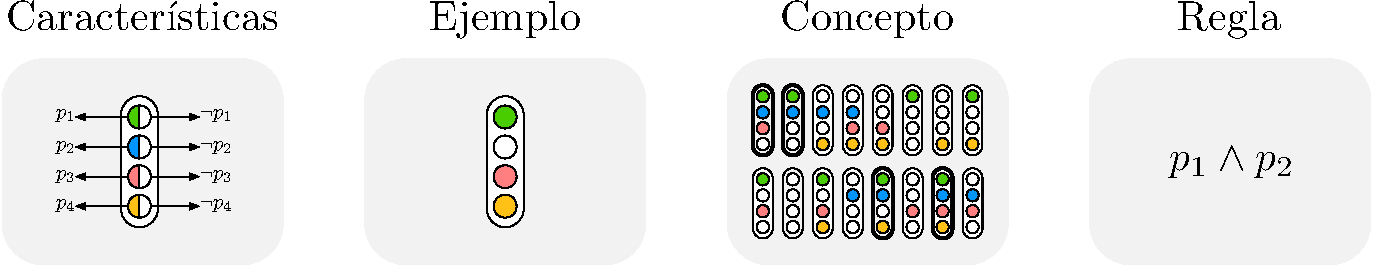
\includegraphics[scale=.6]{../figuras/pre/notacion.pdf}
\widesanti{Sergio, esta imagen es nueva. Pienso que puede dar coherencia con BRM. Puede remplazar a la figura anterior. Hay que actualizar notación en el texto y cambiar $x_i$ por $p_i$, etc. Cuando se presente la figura análoga en BRM, podes mandar un cf. a esta}

%A lower bound for the complexity of a concept in a given logic corresponds to the shortest description of that concept, that is, its minimum description length (MDL).
Un límite inferior para la complejidad de un concepto en una lógica dada corresponde a la descripción más corta de ese concepto, es decur, su longtud mínima de descripción (MDL).

 \begin{figure}[t!]
 \vspace{-0.5cm}
  \centering
  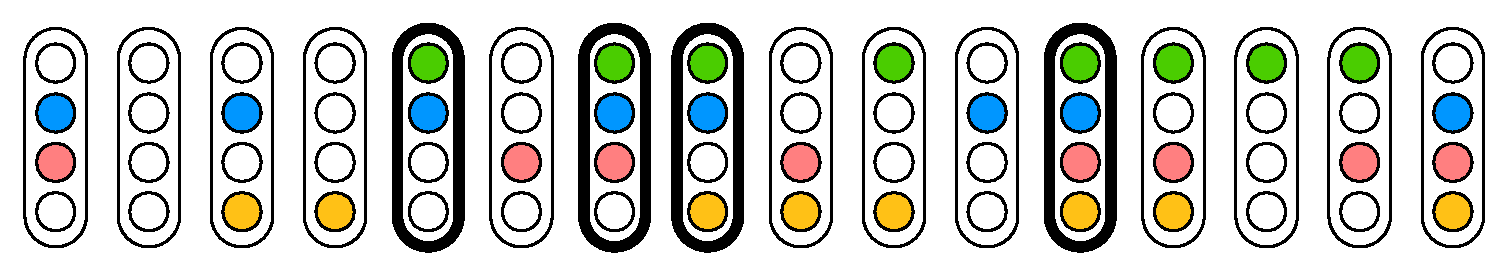
\includegraphics[scale=.335]{semaforos2.pdf}
  %\caption{Example of a concept $\con$, as shown in the experiment. Variables in $\vars=\{x_1,x_2,x_3,x_4\}$ correspond to the presence of a  color light in the object ($x_{1}=$ green, $x_2=$ blue, $x_3=$ red, $x_4=$ orange). Items (valuations) belonging to $\con$ are highlighted with bold border. $\con$ may be described by $x_1\oand x_2$. As in a traffic light, each color is fixed to each position.}
  \caption{Ejemplo de un concepto $\con$, como se muestra en el experimento. Variables en $\vars=\{x_1,x_2,x_3,x_4\}$ corresponden a la presencia de una luz de color en el objeto ($x_{1}=$ verde, $x_2=$ azul, $x_3=$ rojo, $x_4=$ naranja). Los objetos (valuaciones) que pertenecen a $\con$ se resaltan con un bordo en negrita. $\con$ puede describirse mediante $x_1\oand x_2$. Como en un semáforo, cada color está fijado siempre en la misma posición.}
  \label{semaforos}
\end{figure}
   
%The {\em size} of a formula $\varphi$ is denoted $|\varphi|$ and it is defined as the number of operators plus the number of atoms (i.e.\ possibly negated propositional symbols), that is: $|x_i|=|\lnot x_i|=1$ for $i=1\dots 4$ and $|\varphi_1*\varphi_2|=|\varphi_1|+|\varphi_2|+1$ for $*\in\{\oand,\oor,\oxor\}$. For ${\sf L} \in\{\grambool,\gramboolxor\}$ and a concept $\con$ we define the {\em minimum description length of $\con$ with respect to $\mathcal {\sf L}$} as
El {\em tamaño} de una fórmula $\varphi$ se denota como $|\varphi|$ y se define como el número de operadores más el número de átomos (símbolos proposicionales posiblemente negados), es decir: $|x_i|=|\lnot x_i|=1$ para $i=1\dots 4$ y $|\varphi_1*\varphi_2|=|\varphi_1|+|\varphi_2|+1$ para $*\in\{\oand,\oor,\oxor\}$. Para ${\sf L} \in\{\grambool,\gramboolxor\}$ y un concepto $\con$ definimos la {\em la longitud mínima de descripción de $\con$ con respecto a $\mathcal {\sf L}$} como:
$$
\mdl{\sf L}(\con)=\min\{|\varphi|\colon \varphi\in\mathcal L, \sem{\varphi}=\con\}.
$$
Como $\grambool$ es un sublenguaje de $\gramboolxor$, tenemos que $\mdl{\gramboolxor}(\con)\leq\mdl{\grambool}(\con)$ para cualquier concepto $\con$.
   
\paragraph*{Ejemplo.}El concepto $
\con=\{v\colon v(x_1)+v(x_2)=1\},
$
%which expresses that $x_1$ is true or $x_2$ is true but not both can be described in \gramboolxor as $\varphi=x_{1} \oxor x_{2}$, of length 3. In fact, one can check that this is the shortest formula compatible with $\con$, and so $\mdl{\gramboolxor}(\con)=3$. If we now switch to \grambool, we can no longer describe $\con$ as $x_{1} \oxor x_{2}$, since $\oxor$ is not part of its signature. However, in \grambool, the concept $\con$ may be described by  formula $\psi=(x_{1} \oand \neg x_{2}) \oor (x_{2} \oand \neg x_{1})$, of size 7. Since this formula has minimal size, we have that $\mdl{\grambool}(\con)=7$.
que expresa que $x_1$ es verdadero o $x_2$ es verdadero, pero no ambas puede describirse en \gramboolxor como $\varphi=x_{1} \oxor x_{2}$, de tamaño 3. De hecho, se puede comprobar que esta es la fórmula más corta compatible con $\con$, por lo que $\mdl{\gramboolxor}(\con)=3$. Si ahora cambiamos a \grambool, ya no podemos describir a $\con$ como $x_{1} \oxor x_{2}$, dado que $\oxor$ no es parte del lenguaje. Sin embargo, en \grambool, el concepto $\con$ puede describirse mediante la fórmula $\psi=(x_{1} \oand \neg x_{2}) \oor (x_{2} \oand \neg x_{1})$, de tamaño 7. Dado que esta fórmula tiene tamaño mínimo para ese concepto en \grambool, tenemos que $\mdl{\grambool}(\con)=7$.

\section{Experimento}


\renewcommand*{\arraystretch}{1.2}
   
\begin{table*}[!ht]
\vspace{-0.5cm}
\centering

\begin{tabular}{|c|l l | c | c |l l | c | c|}
\hline
                                   &
\multicolumn{2}{c|}{\textbf{Grupo objetivo}}       &
\textbf{$\mdl{\gramboolxor}(\con)$} &
\textbf{$\mdl{\grambool}(\con)$} &
\multicolumn{2}{c|}{\textbf{Grupo control}}  &
\textbf{$\mdl{\gramboolxor}(\con)$} &
\textbf{$\mdl{\grambool}(\con)$} 
 \\ \hline
\multirow{4}{*}{\parbox[t]{2mm}{\rotatebox[origin=c]{90}{\bf Entrenamiento}}} & \targeta & $x_{i}$             & 1 & 1                                                                  & \multicolumn{4}{c|}{$\longleftarrow$Ídem}                                                            \\ \cline{2-9}
                                   &\targetb& $x_{i} \oxor x_{j}$       & 3 & 7 &\controlb& $x_{i} \oor x_{j}$  & 3 & 3                                                                  \\ \cline{2-9}
                                  &\targetc & $x_{i} \oxor x_{j} \oxor x_{k}$ & 5 & 19 &\controlc& $x_{i} \oor (x_{j} \oand x_{k})$  & 5 & 5 \\ \cline{2-9}
                                  &\targetd& $x_{k} \oxor x_{l}$       & 3 & 7&\controld&$x_{k} \oor x_{l}$  & 3 & 3                                                                  \\ \hline
\multirow{2}{*}{\parbox[t]{2mm}{\rotatebox[origin=c]{90}{\bf Evaluación}}}  &\testa& $x_{i} \oand (x_{j} \oxor x_{k})$ & 5 & 9                 & \multicolumn{4}{c|}{$\longleftarrow$Ídem}                                                                                    \\ \cline{2-9}
                               &\testb& $x_{i} \oand (x_{j} \oor x_{k})$  & 5 & 5         & \multicolumn{4}{c|}{$\longleftarrow$Ídem}                                                                                            \\ \hline
\end{tabular}

\caption{Secuencia de conceptos presentados en el experimento: \targeta, \targetb, \targetc, \targetd, \testa, \testb para el grupo objetivo y  \controla, \controlb, \controlc, \controld, \testa, \testb para el grupo control. Cada concepto $\con$ está representado por una fórmula mínima $\varphi$ tal que $\sem{\varphi}=\con$. %Numbers $n/m$ on the right indicate $n=\mdl{\gramboolxor}(\con)$ and $m=\mdl{\grambool}(\con)$.
%MDL is measured as the number of operators and variables (excluding the \textit{not} operator) of the minimal formula with respect to the specified CFG.
}
\label{conceptos}
\vspace{-0.4cm}
\end{table*}

\widesanti{Unifiqué notacion de conceptos con BRM}

55 participants participated in the experiment over the world wide web using the Amazon Mechanical Turk crowd sourcing platform. All were US residents over the age of 18 and had more than 95\% of past tasks successfully approved by other requesters. 44 participants completed the experiment through all the stages and declared not cheating (using pen, screenshots or a similar method to copy the answers) at the end of the experiment. Only data from these participants were used in the analyses reported below.\footnote{The learning times of all participants can be found in https://figshare.com/s/04d338adbbc4b1e83bf0.}

Participants were divided randomly into a control group ($N=21$) and a target group ($N=23$). Both groups were presented with different sequences of six concepts. For each concept, there was a learning phase, a testing phase and a feedback phase. The average time spent in each concept was 167$\pm$20 s.e.m.\ seconds, and the average duration of the task was 21$\pm$4 s.e.m.\ minutes. After moving through the learning, testing and feedback phase of each of the six concepts, participants were asked if they used a pen or recorded the screen information in any way. They were also told that the answer to this question will not affect their payment, but that it was crucial for the experimenters to know.


During the learning phase, all 16 items were presented in the screen (in random order), and items belonging to the concept were identified with bold boundaries, as shown in  Fig.~\ref{semaforos}.
Participants were told that only the items with bold boundaries were `blickets' (or `tufas', etc.: we used different words for each concept in the sequence), and asked them to try to identify what a blicket was. During the testing phase, the 16 items were shuffled in the screen, and participants were asked to click on items that were blickets. If they made mistakes after submitting their answer, they were directed to the feedback phase, in which items that were incorrectly classified were indicated with a red cross. After having studied the feedback, participants were redirected to the testing screen, where items were reshuffled. When every item was correctly classified, participants were asked to give a verbal description of the concept and then continued on to the following concept after a resting period. We characterize the subjective difficulty of each concept as the time the participant spent in learning, testing and feedback phases for that concept (excluding the time spent in the verbal description).


\begin{figure}
\begin{center}
  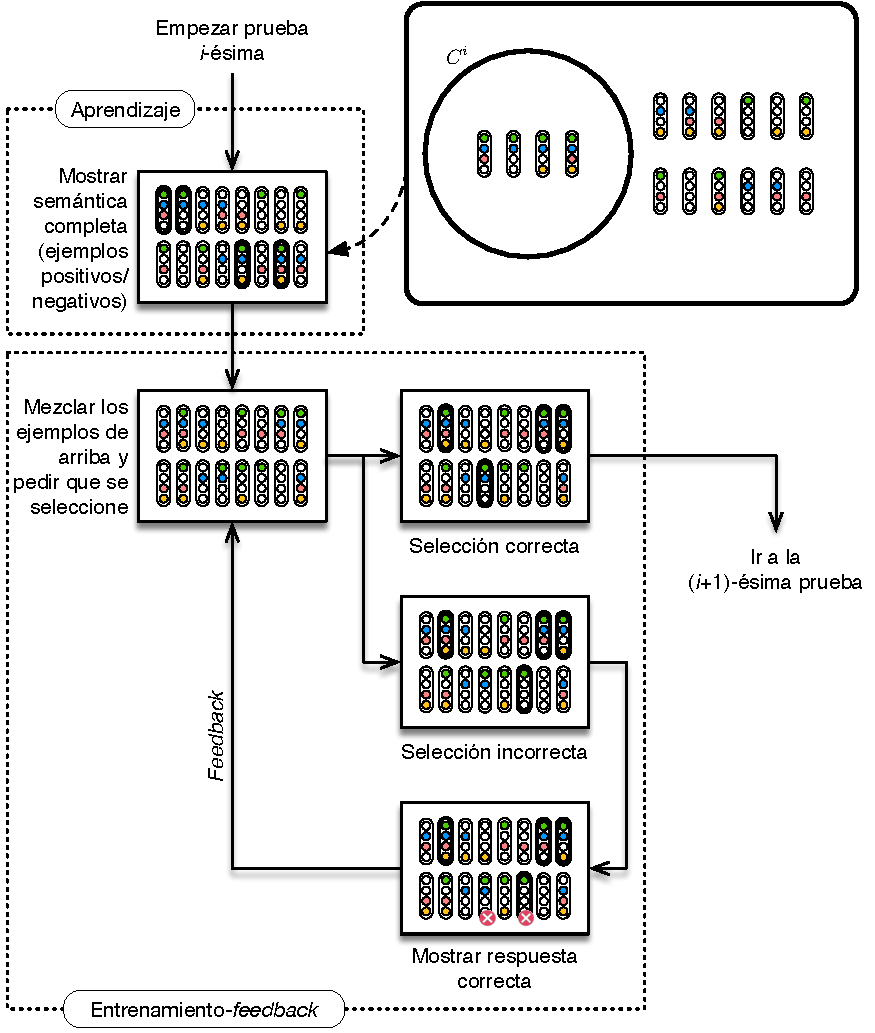
\includegraphics[scale=1]{../figuras/pre/experimento_PRE.pdf}
\end{center}\caption{}
\end{figure}
\widesanti{Sergio, esta figura es nueva. Es una adaptación de la de BRM, más simple y con los ejemplos de semáforos. Pienso que puede dar más coherencia a la tesis. Podés confrontarla desde el capítulo de BRM y decir que en BRM es más complejo: (a) mostramos semantica INCOMPLETA (b) hay 2 conceptos en vez de 1 y (c) hay una etapa de GENERALIZACION}

Both groups (target and control), were exposed to 6 concepts. The second, third and fourth concepts are {\em training} concepts, and were different between both groups. The last two concepts are the {\em test} concepts, and were the same for both groups. The first concept was the trivial concept $x_i$ for both groups, which was aimed to get participants started in the task. Importantly, variables (i.e. color lights inside objects in Fig.~\ref{semaforos}) were randomized for every concept, so paying selective attention to a specific variable across subsequent concepts was not beneficial for learning the concept sequence.


As shown in Table~\ref{conceptos}, we presented the target group with training concepts which are succinctly described when $\oxor$ is part of the language, but necessarily described with lengthier formulas if $\oxor$ is absent; more technically, concepts for which $\mdl{\gramboolxor}$ is much smaller than $\mdl{\grambool}$. We also corroborated that for \targetb, \targetc, \targetd and \testa the number of formulas in $\gramboolxor$ with length strictly smaller than $\mdl{\grambool}$ was at least 10 times greater than the number of formulas in $\grambool$ with length equal to $\mdl{\grambool}$.

Participants in the control group, on the other hand, experienced a sequence of concepts that could be easily described using the language given by \grambool. After these training concepts, both groups were presented with the same pair of test concepts: one which could be only succinctly described in \gramboolxor, and one for which the MDL did not depend on the underlying language \gramboolxor or \grambool. We compared learning times between the two groups for these last two concepts.


As shown in Table~\ref{conceptos}, training concepts for the target (xor) group were: $x_{i}$, $x_{i} \oxor x_{j}$, $x_{i} \oxor x_{j} \oxor x_{k}$, and $x_{k} \oxor x_{l}$, called \targeta, \targetb, \targetc and \targetd respectively. Training concepts for the control group were: $x_{i}$, $x_{i} \oor x_{j}$, $x_{i} \oor (x_{j} \oand x_{k})$, and $x_{k} \oor x_{l}$ called \controla, \controlb, \controlc and \controld respectively. We use the indexes \textit{i, j, k, l} instead of numbers because variables were randomized in each trial. $x_{i}$ could stand for $x_1$, $x_2$, $x_3$ or $x_4$, that is, for any of the four colors. After these four concepts, both groups were presented with the same test concepts: $x_{i} \oand (x_{j} \oxor x_{k})$, and $x_{i} \oand (x_{j} \oor x_{k})$, called \testa and \testb respectively.

Choosing which concepts to show the target group in order for them to `learn' the $\oxor$ operator is critical in our experiment. Crucially, the learner must have an option between two alternatives that describe the concept: one that is succinct but uses $\oxor$, or necessarily a much longer one in the absence of $\oxor$. In other words, these concepts must be compatible with short logical formulas if and only if we take \gramboolxor as the language of description. To ensure that this was the case, we enumerated, for each concept, all formulas compatible with it and produced by the \grambool and \gramboolxor grammars up to length 19. For all training concepts of the target group, the shortest compatible formula without $\oxor$ is much longer than the shortest compatible formula with $\oxor$. This is shown in Table\ref{conceptos}.

\section{Model-Free Results}

We measure the subjective difficulty of a given concept as the total time needed by the participant to successfully encode the concept, which indicates that they can reliably express which exemplars belong to the concept and which do not.

Participants from the target group spent almost half the time than participants from the control group in \testa, which could be succinctly described only in \gramboolxor ($111\pm16$ s.e.m.\ seconds versus $214\pm37$ s.e.m.\ seconds, a two-sample t-test reveals $t_{42}=2.6$, $P<0.01$), as shown in Fig.~\ref{model free} (a). We also found that the control group learned much faster \testb ($143\pm14$ s.e.m.\ seconds for the target group versus $76\pm10$ s.e.m.\ seconds for the control group, $t_{42}=3.5$, $P<0.01$). A mixed ANOVA with \testa-\testb as within subject factor and target-control groups as between subject factor reveals a strong interaction between group and \testa-\testb ($F=15.3$, $P<0.001$), indicating that the differences in learning times for \testa and \testb were very different between the two groups.

The target group encoded \testa more efficiently than the control group. We propose that the control group expected to find in \testa and \testb structures that could be easily built in \grambool. The target group, on the other hand, became biased towards the $\oxor$ structure, and they expected to find it in \testa and \testb. This caused \testa to be encoded more rapidly by the target group and \testb more rapidly by the control group. Assuming that the subjective difficulty of learning a concept is proportional to the complexity of its internal representation, we conclude that after exposure to the training concepts, participants in the target group represented the $\oxor$ more efficiently than the control group, and expected to find this structure in \testa and \testb.



\begin{figure}[t!]
      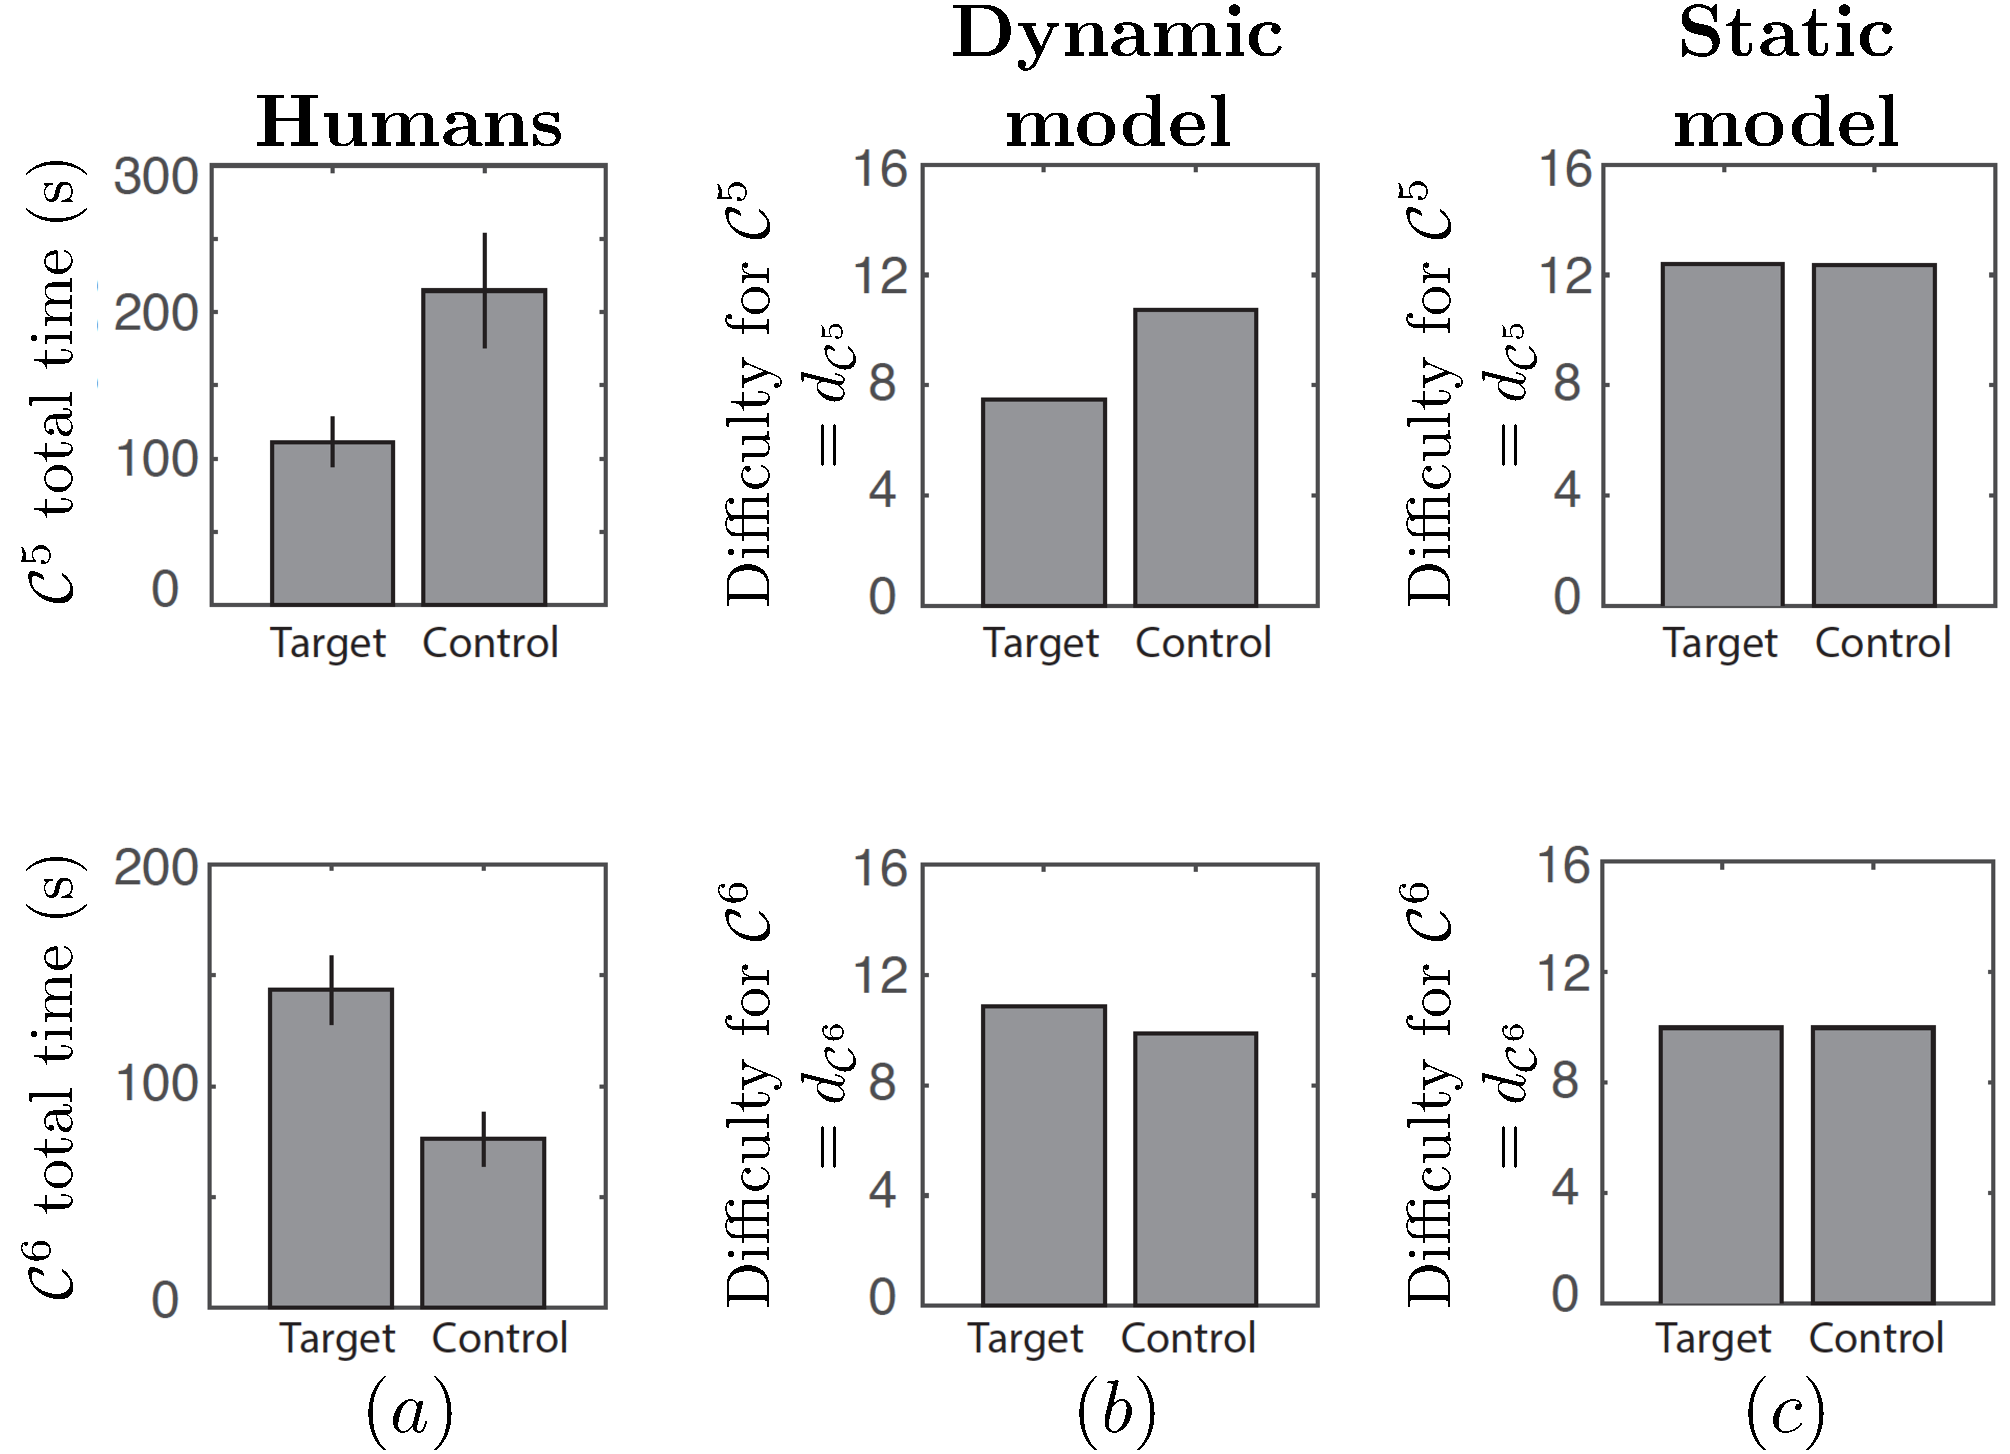
\includegraphics[scale=0.25]{model_free-3.pdf}
      \centering
      \caption{Concept learning time $(a)$ and difficulty predicted $(b)$, $(c)$ for the two test concepts (\testa and \testb). Error bars are s.e.m.\ across subjects.}
      \label{model free}
   \end{figure}
   
\section{Model}

When presented with a concept (e.g.~Fig.~\ref{semaforos}), our model generates logical formulas and evaluate them to true or false for that concept, keeping the formula only if it is true. To generate formulas, the model uses a symbolic language in which each rule (symbols and operators) is associated with a probability of being used. The probability of generating a formula is proportional to the product of the probabilities of the rules required for building it, and therefore it decreases exponentially with its length. Furthermore, if one of the rules has a very low probability of being used, formulas that require it will also have very low probability.

The \textit{Static model} maintains the rules' probabilities fixed throughout the concept sequence (the 6 concepts in Table~\ref{conceptos}). The \textit{Dynamic model} updates the probabilities after each concept, in order to minimize the expected description length of future concepts, assuming they have similar structure to the concepts learnt so far. We include in this model the $\oxor$ rule a priori in the language, but with vanishing probability of being used. Changes in this probability can be analogously interpreted as the probability that a rational agent without the compiled symbol a priori decides to add the compiled expression as a new primitive into her language. %This means that our model will fit somewhere between the computational and the algorithmic level of analysis by Marr's \cite{marr1979computational,griffiths2015rational}. It can explain algorithmically how learning occurs, however, adding a new primitive is not modeled entirely at this level. The vanishing probability analogy is sufficient to make the new primitive be highly unlikely to be used without exposure and to allow it to emerge after concepts. Still, it does not explain --at an algorithmic level-- how any new primitive can arise, leaving the mechanics of the language change between the computational and algorithmic level.


\subsection{Static Model}

\newcommand{\form}{\varphi}
Under the LoT assumption,  given a concept $\con$ (e.g.\ Fig.~\ref{semaforos}), the probability that an agent uses formula $\form$ to explain this concept is defined by Bayes theorem: 
$$
P(\form\mid \con) \propto P(\con\mid \form)P(\form).
\label{Bayes fix}
$$
% \begin{equation}
% P(\form\mid \con) \propto P(\con\mid \form)P(\form).
% \label{Bayes fix}
% \end{equation}
%
The likelihood $P(\con\mid \form)$ of a logical statement $\form$ can be simply defined as 1 if $\sem{\form}=\con$ and 0 otherwise. In other words, for any given concept, only explanations that describe this concept are considered as possible explanations. The likelihood term has been defined more flexibly in the literature~\cite{goodman2008rational,piantadosi2016logical}, allowing for mislabeled elements. We keep this simpler definition in order to reduce the number of free parameters of the model, as we do not intend to account for mislabeling errors in our experiment.

The prior $P(\form)$ is defined by augmenting the context-free grammars shown in Fig.~\ref{PCFG} into a probabilistic context-free grammars (PCFG). In the PCFG, each rule has associated a parameter indicating the probability of using that rule. A PCFG can be used to produce logical statements similar to a CFG. Each non-terminal remaining in the statement is expanded using a rule of the PCFG with probability proportional to that rule's associated parameter, until no non-terminals remain in the statement. 

We assume that the probability that a subject uses formula $\form$ to explain concept $\con$ is proportional to the posterior $P(\form \mid \con)$, and the subjective difficulty $d_\con$ of a concept $\con$ to a participant is proportional to the length of the formula that the participant is using to explain that concept. However, there is no way to know directly which internal formula $\form$ the participant is using (and therefore we do not know $|\form|$). Hence, the most parsimonious approach is to consider the entire posterior distribution $\textbf{P}(\form \mid \con)$ over possible formulas.\footnote{This is equivalent to the Sampling Hypothesis described in~\cite{denison2013rational}, by which participants represent distributions through samples. Similar results are obtained if each participant carries entire probability distributions.}

Given a concept $\con$, the expected length $E_\con$ of the formulas used by the participant is simply
%
 \begin{equation}
E_\con=\sum_{\sem{\form}=\con} |\form| \ P(\form \mid \con),
 \label{expected length}
 \end{equation}
%
where the sum is over all formulas $\varphi$ compatible with $\con$. We  define the difficulty $d_\con$ of a concept experienced by the participant  as $$d_\con \propto E_\con + \alpha N_\con,$$
%
% \begin{equation}
%d_\con \propto E_\con + \alpha N_\con,
% \label{length}
% \end{equation}
%
where we added a term that accounts for the cardinality of the concept: $N_\con$ is the cardinality of the concept or its complement, the one being smaller, i.e.\ $N_\con=\min \{ \#\con, \#\overline \con\}$ (e.g.\ $N_\con=4$ for the concept $\con$ of  Fig.~\ref{semaforos}), and $\alpha$ is a free parameter fitted globally for all concepts and participants to its maximum likelihood value of 0.9. In this way, we remove the asymmetry between positive and negative examples, while accounting for the toil taken by considering a larger number of items simultaneously.

In practice, to approximate $E_\con$ for each concept $\con$, we calculated the posterior probability $P(\form\mid \con)$ of all compatible formulas $\form$s up to size 19 with $P(\form\mid \con)$ and then use ~\eqref{expected length}. Since the space of all possible $\form$s grows exponentially with $|\form|$, normative procedures for estimating $P(\form\mid \con)$ in this space involve stochastic search algorithms. However, in our case, we were able to exhaustively enumerate and calculate the posterior probability of \textit{all} formulas generated by the PCFG up to a sufficiently high size $M$ such that all formulas with $|\form|>M$ have vanishing probabilities when compared to shorter compatible formulas for the current concept (because the prior $P(\form)$ decreases exponentially with the size of the formula).

\subsection{Dynamic Model}

Up to this point, we assumed that, given a concept $\con$, the posterior distribution over formulas $P(\form\mid \con)$ was independent of the other concepts presented in the sequence. However, if the LoT (i.e. the PCFG) updates with experience, the prior $P(\form)$ in $P(\form\mid \con)$ will change, and so will $E_\con$ in \eqref{expected length} and finally the subjective difficulty $d_\con$. Therefore, $d_\con$ will depend on the sequence of concepts that were previously presented to the participant.

In other words, since now $P(\form)$ depends on the sequence of concepts experienced by the participant, instead of $P(\form\mid \con)$, we have $$P(\form\mid \con^{t},\dots,\con^{1}) \propto P(\con^{t}\mid \form)P(\form\mid \con^{1},\dots,\con^{t-1})$$, 
% \begin{equation}
% P(\form\mid \con^{t}) \propto P(\con^{t}\mid \form)P(\form\mid \con^{1},\dots,\con^{t-1}),
% \label{Bayes}
% \end{equation}
%
where $\con^{t}$ is the concept presented at trial~$t$, and $P(\form\mid \con^{1},\dots,\con^{t-1})$ depends on the state of the PCFG at trial $t$, which in turn depends on how the PCFG gets updated from trial to trial.

Intuitively, the update process increases the probability of using a certain rule in the PCFG accordingly to how useful this rule was to compress compatible formulas for the concepts previously learned in the same domain. Specifically, we model the update process in a normative manner: the probability of using a rule of the PCFG at trial $t$ is equal to the Bayesian posterior probability that this rule will enable the learner to find compressed explanations at trial $t$, according to how useful it was to compress explanations in trials $1,\dots,t-1$.

To formalize the update of the PCFG, we define $P(\form)$ similarly to~\cite{goodman2008rational}. Specifically, the prior probability of a logical statement at trial $t$ in the concept sequence uses a single Dirichlet-multinomial for the set of rule expansions. The Dirichlet is parameterized by a set of positive real numbers $D_{i}^{t}$, one for each rule $i$ in the PCFG, which in turn determine the probability of using rule $i$ at trial $t$: a higher $D_{i}$ indicates a higher probability of using rule $i$.

The prior is specified by the set Dirichlet parameters $\textbf{D}^{0}$ with which we start the experiment ($\textbf{D}^{0}$ represents a vector containing the prior parameters of all rules in the grammar at trial 0). In our experiment, we set the prior Dirichlet parameters of all rules equal to 1, and the parameter of the rule that expands the target operator to a value several orders of magnitude smaller ($\approx 10^{-4}$). This means that the target operator was practically absent at the beginning of the experiment, but it was technically possible to `learn it' by increasing its probability as the experiment developed.

Under the Dirichlet model, the prior $P(\form\mid \con^{1},\dots,\con^{t-1})$ can be rewritten using the Dirichlet parameters as $P(\form\mid\textbf{D}^{t})$. Therefore, to know how $P(\form\mid \con)$ updates from trial to trial, we only need to know how $\textbf{D}$ updates from trial to trial.

The Dirichlet parameter of rule $i$ at trial $t+1$ is equal to its parameter at trial $t$ plus the amount of times the production $i$ was used in generating all formulas compatible with the concept at trial $t$ (we note $M_{i}(\form)$ as the number of times that rule $i$ is used in generating formula $\form$), weighted by each formula's posterior probability at trial $t$:
 \begin{equation}
 D_{i}^{t+1}=D_{i}^{t}+\sum_{\sem{\form}=\con^t} P(\form\mid \textbf{D}^{t}) \ M_{i}(\form).
 \label{Dirichlet}
 \end{equation}
 %
This Bayesian learning mechanism increases the probability of using rules that allow concepts to be succinctly described. This happens because these formulas have higher probability $P(\form\mid \textbf{D})$ than longer formulas, so the Dirichlet parameters of the rules that build these formulas increase more strongly than those of the rules that build longer formulas.   

\section{Results}

The Bayesian agent that minimizes the expected complexity of future concepts by optimally adapting its LoT to the inferred structure of the task accurately captures the dynamics of human learning across concepts. If we did not allow the model to update the probability of the operators after each concept, and particularly the compiled operator $\oxor$, the control group and the target group would be indistinguishable to the model as it would predict equal average formula length for both groups (see Fig.~\ref{model free}, {\em Static Model}). Instead, as shown in Fig.~\ref{results}, by adjusting the prior probabilities based on concept exposure the dynamic model is able to capture learning time patterns in the target groups ($R^{2}=0.96$ compared to $R^{2}=0.73$ for the static model). Expectedly, both models perform similarly in the control groups as they were designed to not encourage the use of any particular operator ($R^{2}=0.72$; $R^{2}=0.71$ for the static model). The impact of the learning capability of the model is most evident in the target group concept sequence, which was designed to this effect. If the structure of the concepts does not bias the LoT primitives one way or the other, it is expected that a static model will provide a reasonable fit. However, it is difficult to tell a priori how unbiased a set of concepts really is, so experiments relying on repeated concept exposure should always take between-concept learning into account.

Allowing the model to constantly update its beliefs from concept to concept is a requisite to capture human learning times. We now explain how the pattern of subjective difficulties in Fig.~\ref{results} emerged in the \textit{Dynamic model}. In this scenario, learning for the model is formalized by the update of rule parameters from concept $t$ to concept $t+1$ according to \eqref{Dirichlet}. In Fig.~\ref{evol} we show how this learning takes place in the concept sequence for the target group. There are mainly two competing formulas when \targetb is presented: $x_{i} \oxor x_{j}$ and $(x_{i} \oand \neg x_{j}) \oor (\neg x_{i} \oand x_{j})$. Given the low a priori value of the parameter of the $\oxor$ rule, the posterior of the formulas of type $(x_{i} \oand \neg x_{j}) \oor (\neg x_{i} \oand x_{j})$, which do not use the $\oxor$ operator, is much higher than the posterior of $x_{i} \oxor x_{j}$. Therefore, in Fig.~\ref{results} we see a large predicted difficulty by the dynamic model for this concept (since the posterior lies mainly over these longer formulas without $\oxor$, see  \eqref{expected length}). 

\begin{figure}
      \centering
      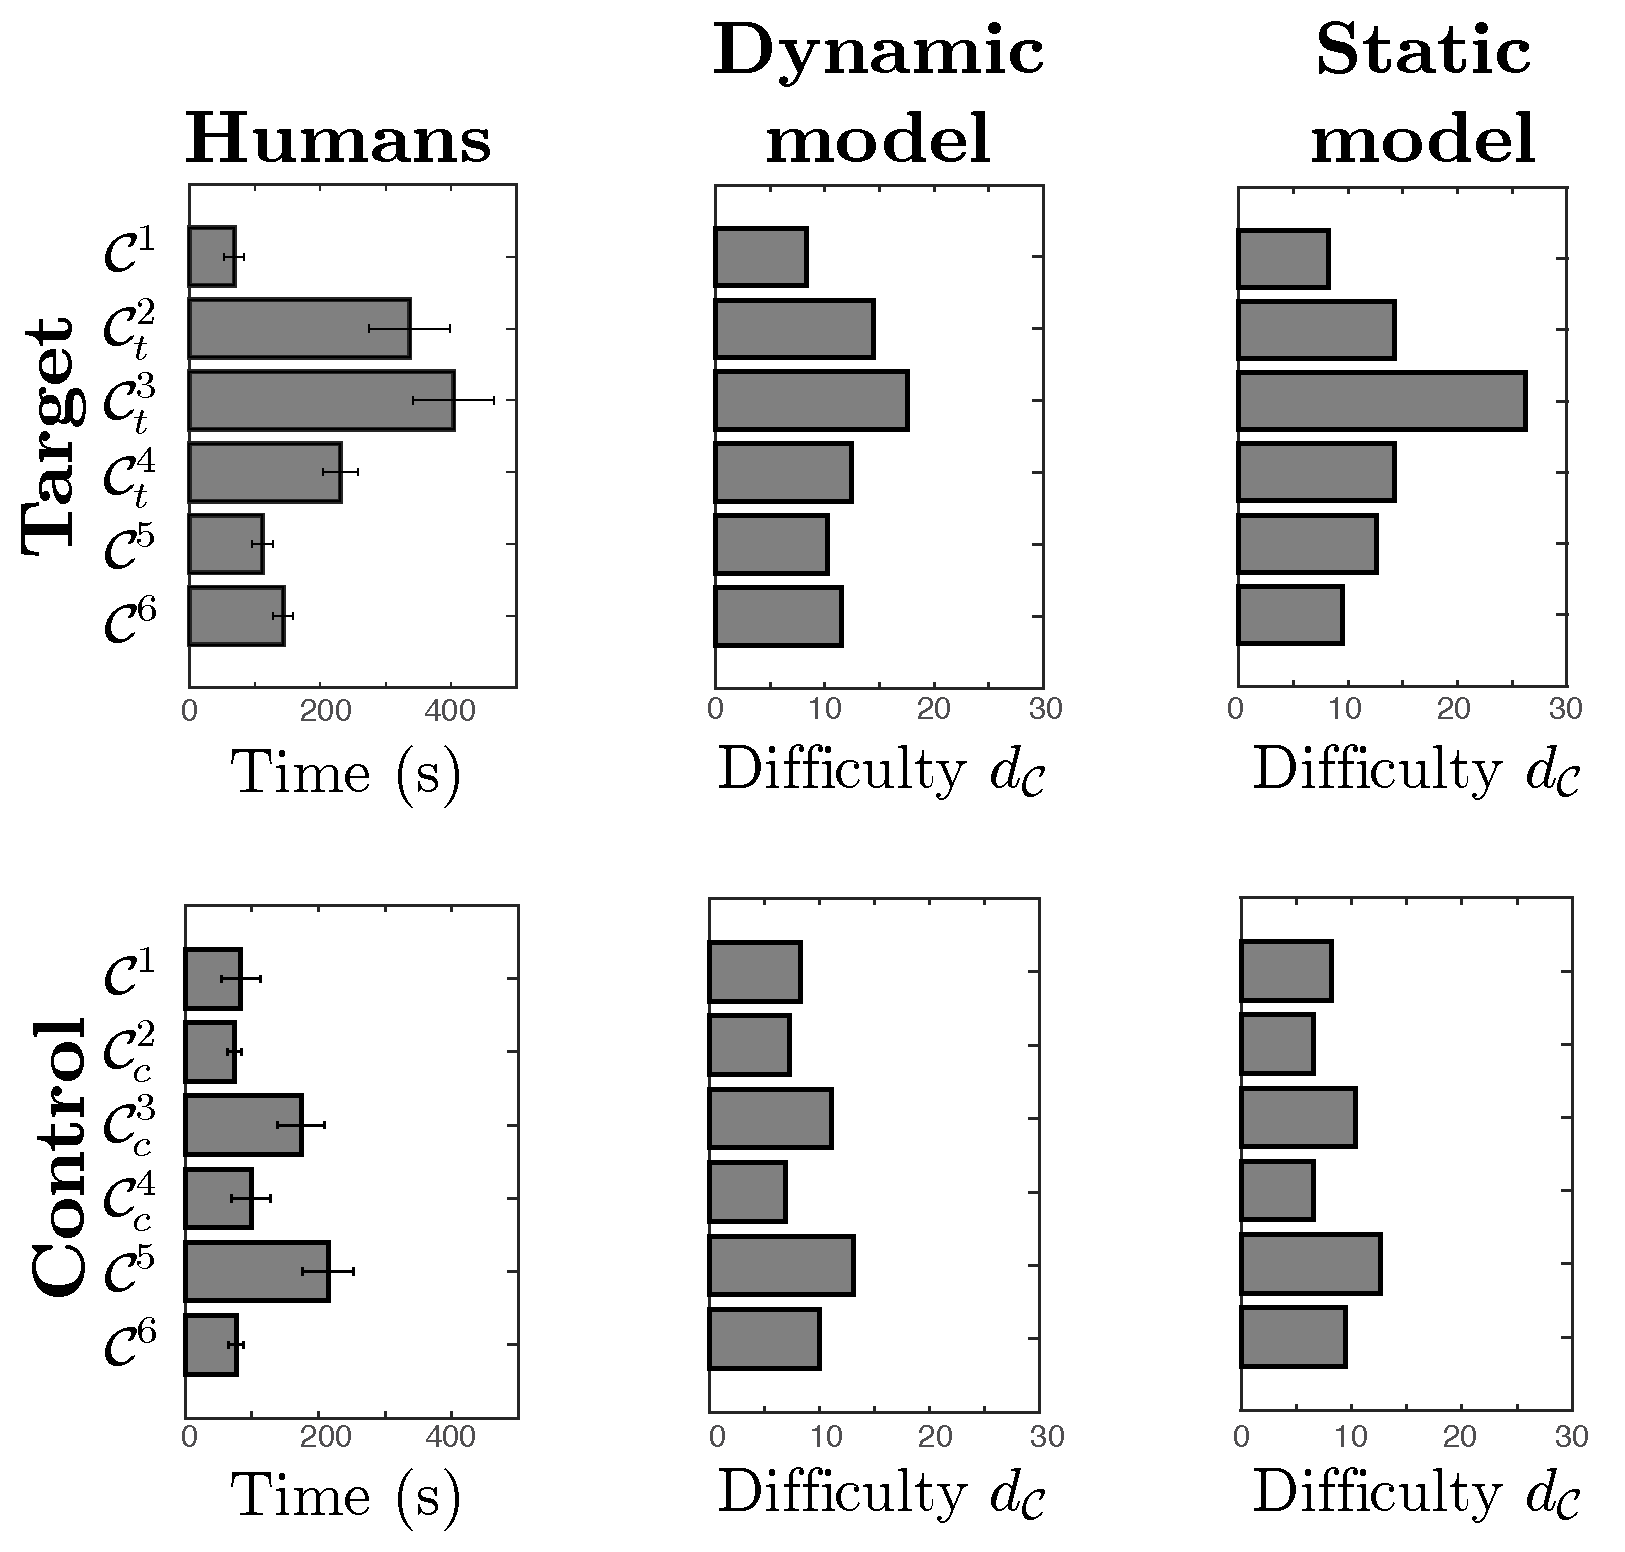
\includegraphics[scale=.30]{results-3.pdf}
      \caption{Learning times and model predictions for target and control groups (see Table~\ref{conceptos} for concept details). The predicted difficulties of each model were calculated using $d_\con$. Error bars are s.e.m.}
      \label{results}
\end{figure}

\begin{figure}
        \centering
        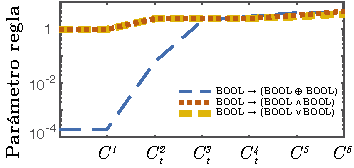
\includegraphics[scale=1]{dirichlet_evol-2.pdf}
        \caption{Evolution of Dirichlet parameters of different rules after each concept experienced by the target group.}
       \label{evol}
\end{figure}\santi{aca hay alguna diferencia de nomenclatura de conceptos. Prefier llamarlos $C^1, C^2$, o lo que sea igual a BRM}


However, the little increment in the $\oxor$ rule after \targetb (see Fig.~\ref{evol}) is sufficient for making the formula $x_{k} \oxor x_{l}$ to have higher relative posterior in the next concepts, making the increment in the parameter of the $\oxor$ rule much greater than before. Additionally, the difficulty inferred by the model is much smaller the second time the concept is presented (compare \targetd and \targetb concepts in Fig.~\ref{results}), since now the posterior is more evenly distributed between long (without $\oxor$) and short (with $\oxor$) formulas (see Eq. \eqref{expected length}). Finally, when the concept \testa is presented, the learner has completely compiled the $\oxor$ rule into her language, ascribing the formulas that use the $\oxor$ operator a much higher posterior probability relative to the long formulas that do not use the $\oxor$ operator. Therefore, the inferred difficulty for \testa is much smaller than those describing previous concepts, almost as simple as concept \targeta (see Fig.~\ref{results}).

Finally, the strong $\oxor$ acquired by the target group increases the difficulty of \testb relative to the control group (see Fig. 3). This occurs because there are several formulas of length 9 that use the $\oxor$ operator (around 6000), significantly increasing the expected difficulty of the concept (see Eq. \eqref{expected length}). For the control group, the posterior probability of these formulas is very low, causing a smaller increase in the expected difficulty.

The previous results point to a competition between different rules in the grammar. In our model, competition between $\oxor$ and the other operators is modulated by the initial relative value of the Dirichlet prior of the $\oxor$ rule, and the overall magnitude of the priors of all rules. The initial $\oxor$ prior measures how useful $\oxor$ should be (relative to the other rules) in order to increase the likelihood of using it in the future. If the $\oxor$ prior is too low relative to the priors of other rules, then formulas with $\oxor$ must be much shorter than formulas without $\oxor$ in order for them to have appreciable posterior and increase the $\oxor$ parameter in Eq. \eqref{Dirichlet}. In our experiment, if the prior is smaller $10^{-12}$ (and 1 for all other rules), then the predictions of the dynamic and static model for the target group are approximately equal: the advantage of using $\oxor$ in the target concepts is not enough to increase the likelihood of using $\oxor$. On the other hand, if the $\oxor$ prior is too high, we cannot model the high difficulty of \targetb for the target group and the high difficulty of \testa for the control group. For example, if the $\oxor$ prior is higher than 0.05 (and 1 for all other rules), the difficulty of \targetb and \targetd are approximately equal (corresponding to the short formula with $\oxor$) and also the difficulties of \testa for control and target groups.

The other free parameter that modulates competition is the overall magnitude of the Dirichlet priors, which determines how many times an efficient rule should be encountered before incorporating it. If the magnitude is too high, then observing a useful rule does not significantly change its Dirichlet parameter relative to the others, eliminating from the model the rapid rule acquisition clearly showed by participants. This happens because in Eq. \eqref{Dirichlet} the magnitude of the updates from $t$ to $t+1$ are at most of order $M$, the number of times that operators appear in formulas with high posterior. In our experiment, if all rules have prior equal to 1 and $\oxor$ has 1/1000 we get similar results to the ones in Fig.~\ref{results}, but if all rules have prior equal to 10000 and $\oxor$ has 10 the additions to the $\oxor$ parameter are insignificant, so the dynamic and static models make the same predictions for the target group.

In our model a large enough exposure to a concepts will increase the Dirichlet parameters without bounds, progressively decreasing learning flexibility. Although our experiment is not long enough to test it, such inflexibility is very unlikely to be true. For example, in the LoT fitting experiment from ~\cite{piantadosi2016logical} they found that human Dirichlet priors for most propositional operators are between 0.3 and 3, instead of orders of magnitude higher (as expected by Eq. \eqref{Dirichlet} after exposure to a large number of concepts). Therefore, a more complete model of lifelong language acquisition should include an extra normalization or forgetting parameter that decreases the overall magnitude of the Dirichlet parameters, preserving the high learning flexibility that we observed in our experiment.


\section{Discussion}

\par We measured the subjective difficulty that participants experience when learning a sequence of concepts. To explain this subjective difficulty, we resource to propositional logic as a  base description language. In the target group we experimented with concepts which can be succinctly described in the base language {\em that also contains an extra operator $\oxor$} for exclusive disjunction but that needed necessarily longer descriptions over the base language (where this operator is absent). On the contrary, the control group is exposed to concepts where $\oxor$ does not help to achieve succinctness.

Learning times are consistent with the hypothesis that participants in the target group smoothly adopt the $\oxor$ as a new primitive of their LoT in order to absorb the concepts they have been exposed to, with no more incentive than decreasing the expected complexity of future concepts. We do not claim that participants have learned the $\oxor$ operator defined by any specific formula using the previous operators, however, their LoT seems to have constructed an operation that matches the semantics of the exclusive or in order to compress such patterns of data and identify them more efficiently.

\par Here, we focus on transfer learning effects when learning sequential concepts that share the same hierarchical structure. We acknowledge, however, that several other transfer learning effects are present in human sequential logical concept learning, such as when subsequent concepts differ in the relevant variables (e.g.\  color lights in our experiment) \cite{blair2009extremely}, when changing the relevant variables in subsequent exclusive disjunctions \cite{kruschke1996dimensional}, or when two categories are learned in an interleaved or a focused manner \cite{carvalho2014putting}. However, unlike superficial knowledge about the task (like the frequency of appearance of different symbols and logical operators in the concept sequence), identifying the latent hierarchical structure of concepts have extremely important computational consequences: it allows for exponentially less complex representations \cite{bengio2013representation,lake2015human}, maximizing the expected value of future computations within resource-bounded constraints~\cite{gershman2015computational}. In our task, in order to focus primarily on the learning process of the $\oxor$ structure, we randomize variables in each trial, such that other kinds of transitions are averaged out across participants. 

\par Most LoT studies provide a language that is fixed once trained or inferred over a specific data. We claim that when a specific language beats a second one at fitting some experimental data, what we may be seeing is an effect of prior experience (including from the experiment itself), more than an intrinsic feature of the LoT. This leads to a fundamental difficulty in trying to experimentally uncover what the actual human symbolic substrate of thought is. Experimental results have shown for instance that a grammar with \textit{and, or}, and \textit{not} better explains Boolean concept learning than one with \textit{nand}, despite both being expressively equivalent~\cite{piantadosi2016logical}.  In our view, this cannot be taken to mean anything more than that in the current state of affairs of the world, the \textit{nand} operator is not very useful for compressing information. We have shown that participants can rapidly compile new expressions in their LoT if they begin to be useful, which emphasizes that one cannot simply ignore the order in which concepts are presented to the participant when studying aspects of the LoT.

When Fodor proposed the Language of Thought hypothesis \cite{fodor1975language}, what he had in mind was a symbolic system we all came equipped with from birth. Stating that this language is in fact always flexible might seem in outright contradiction with Fodor's original idea. In fact, what studies in the LoT literature (including this one) are probably probing is one among many languages in a hierarchy of increasing abstraction. As we progress in life, we find some conceptual summaries useful, and compiled them in a more abstract token. It is even likely that there is no proper hierarchy with sharply defined boundaries between levels, but instead a less organized progression of concepts of increasing abstraction, with thought progressing seamlessly using constructs at different levels. %Further empirical studies of the way we reuse concepts will hopefully pave the way for a broader understanding of human cognition.


\section{Conclusion}

We defined a model to measure the subjective difficulty of learning a sequence of concepts. The model updates the grammar production probabilities between concepts and predicts difficulty as the size of compatible formulas weighted by their posterior probability. This learning mechanism allows to simulate the emergence of a new primitive in the language, as it becomes useful to encode the concepts presented so far. The predicted difficulties strongly resembles the pattern of human learning times in a sequence of concepts that required the $\oxor$ operator in order to be efficiently represented.
